\IEEEPARstart{T}{he} performance of a modern day microprocessor is much higher than that of typical memory. Much of the computational time is thus used to access the memory of the RAM and load it into the CPU. This is a growing bottleneck in a time where microprocessors are still increasing in performance. 

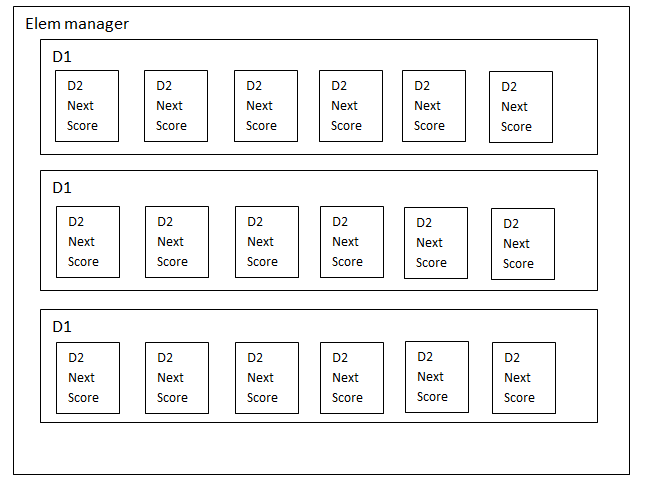
\includegraphics{table3.png}

A prefetcher reduces this bottleneck by predicting which instructions are addressed next. Memory fetches are attempted to be done before the memory is needed by the microprocessor, leading to a decreased time where the processor is stuck in a waiting state. If the prefetched memory addresses differ from what was needed, the processor needs to access the memory anyway. This is the worst case scenario, in which the cache has no effect on performance.

The goal of this project was to make a prefetcher that would increase the performance of a microprocessor. The idea was also to run the prefetcher in a simulator environment with equal hardware specifications for everyone, so that everyone could work with a common interface and the results would be comparable. 

The prefetcher presented in this report is based on pattern recognition implemented as a two dimensional vector structure.
